\chapter{测试与分析}\label{chap:test}

\section{CNN 加速器测试实验环境}

本设计中使用的 CNN 模型是 YOLO V2 Tiny\citep{redmon2017yolo9000};数据集为 VOC 2007 数据集\citep{everingham2007pascal},该数据集包含了 20 个类;FPGA 平台为 PYNQ-Z2 开发板(Dual ARM A9 + FPGA)。

硬件设计工具使用如下:CNN 加速器使用 Vivado HLS 2018.2 工具设计,硬件工程使用 Vivado 2018.2 工具设计;软件设计工具如下:使用 riscv32-unknown-elf-gcc 交叉编译工具对 RISC-V 处理器的程序进行编译。

\section{对比测试环境}

为了直观了解 CNN 加速器的加速效果,设计了3组对照实验进行对比分析,分别如下:

X86架构 CPU 平台:CPU为 Intel i7-9700K,8核心,频率为 4.9 GHz;32GB 运行内存;

嵌入式 CPU 平台:树莓派 3B,CPU 为四核 ARM Cortex-A53,频率为 1.2 GHz;1 GB 的运行内存;

嵌入式 GPU 平台:NVIDIA Jetson Nano,四核 ARM Cortex-A57 MPCore 处理器,频率为 1.43GHz;GPU 为 Maxwell 架构,配备 128 个 CUDA 核心;4GB 运行内存。

\section{CNN 加速器资源消耗评估}

% PYNQ-Z2 开发板上使用的 ZYNQ 7020 芯片有 220 个 DSP 单元,在当前的 CNN 加速器的设计中,卷积过程使用定点 16 位精度的乘法运算,因此每个乘法器会消耗一个 DSP 单元,加法器消耗 LUT,不消耗 DSP。CNN 加速器的运行频率为 150 MHz,因此可以计算出本系统的性能上限为 66GOPS($220 \times 150 \times 2 / 1000 = 66$)。

% PYNQ-Z2 开发板上的内存型号为 32bit DDR3-1066,理论最大带宽为 4.26 GB/s;由 UG585 \citep{xilinx2015zynq} 可知,实际上带宽利用率为总带宽的 75 \% 左右,所以本系统的最大带宽为 3.198 GB/s。根据文献 \citep{陈辰2019基于}中的计算可知,在兼顾性能与功耗的情况下,选取设计参数为:$Tif=2,Tof=86,Toy=26,Tox=36$,在使用该参数的情况下,CNN 加速器的算力为 30.33 GOPS。

整个异构运算系统的设计连接如图~\ref{fig:VivadoStructure}所示,其中 YOLOV2\_FPGA 为基于 YOLO V2 算法的设计 CNN 加速器 IP 核。RISCV\_Processor 为 RISC-V 处理器 IP 核。其余部分是 SOC 中的一些基本外设。YOLO V2 算法加速器有 1 个 AXI-Lite Slave 接口,连接在 RISC-V 处理器的数据总线接口上,负责状态寄存器的控制;还有 5 个 AXI Master 接口分别与 DDR 的 HP[0:3] 接口连接,其中有两个 AXI Master 接口连接在 HP[3] 上。CNN 加速器及其数据通路运行在 150 MHz 的时钟频率下,SOC 中其他部分运行在 100 MHz 的时钟频率下。

\begin{figure}[!htbp]
    \centering
    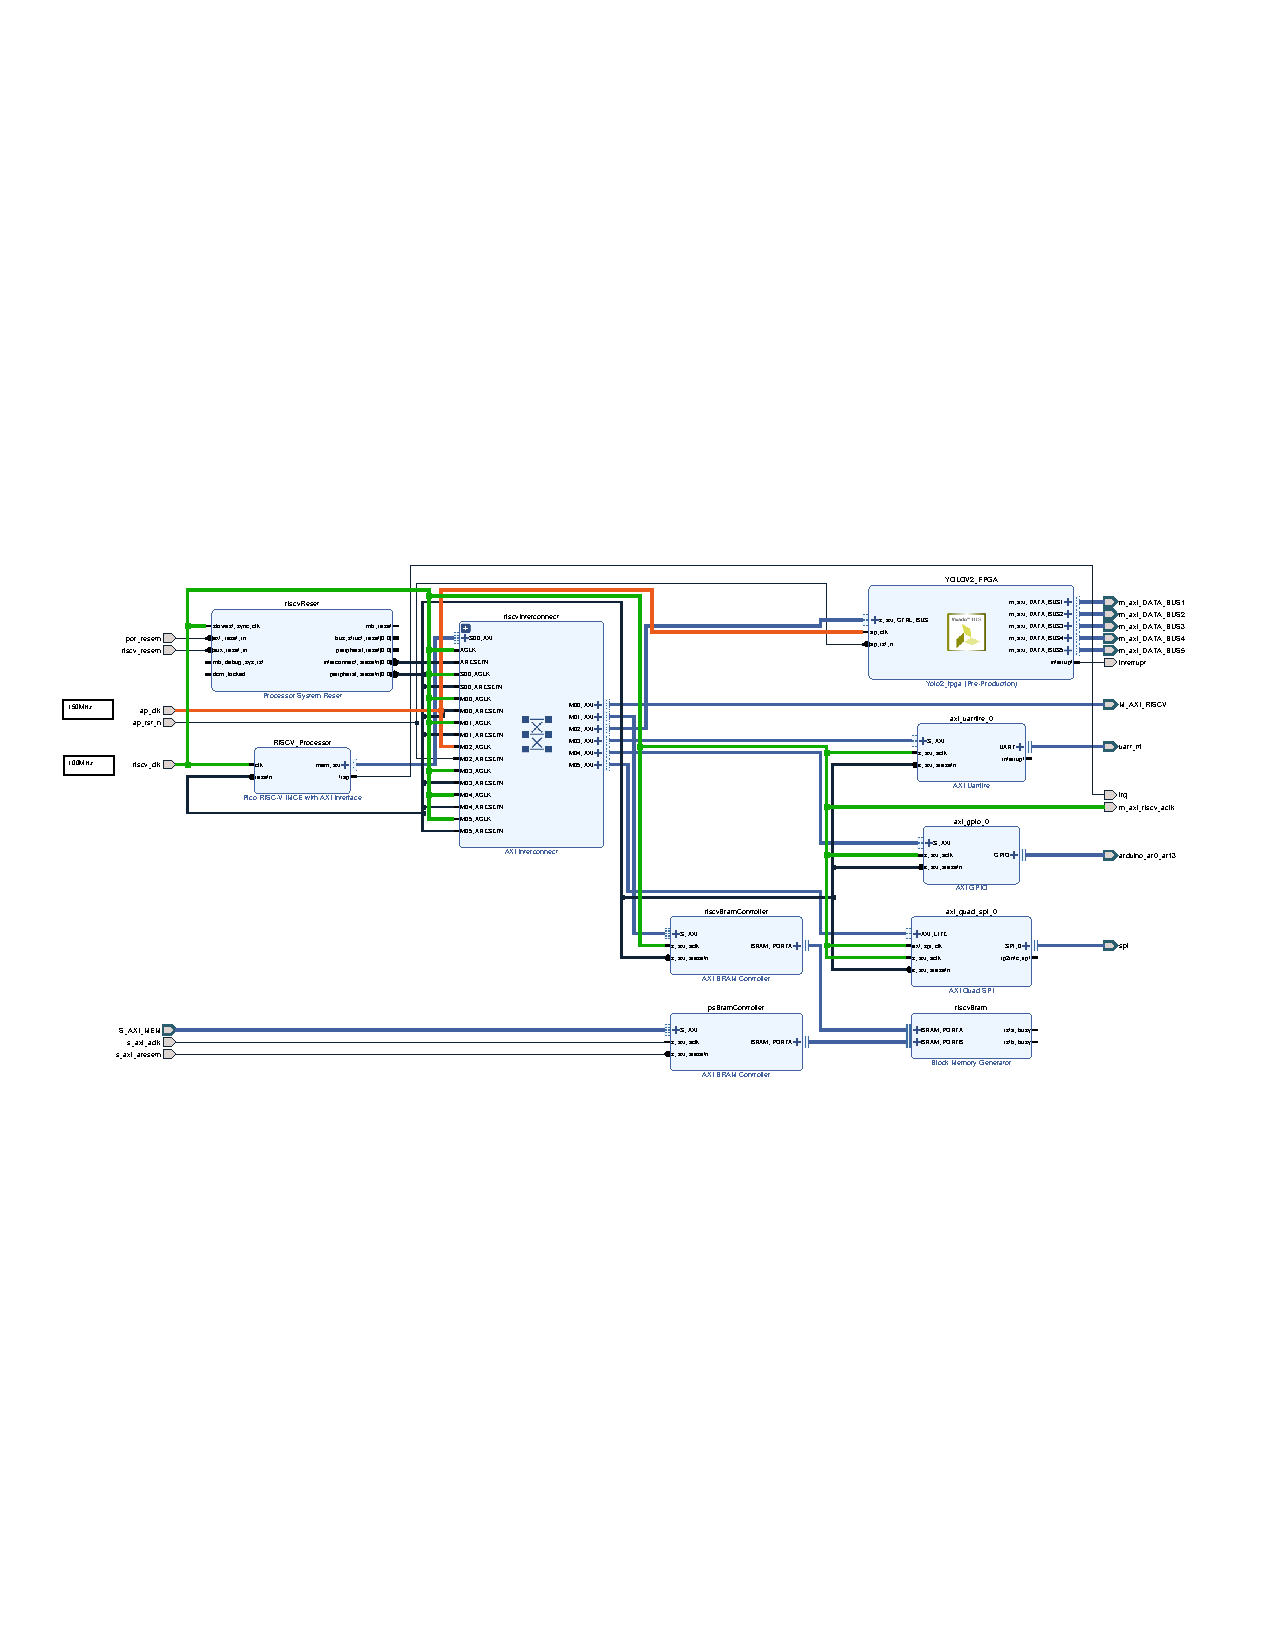
\includegraphics[width=1.0\textwidth,trim=20 270 20 270,clip]{VivadoStructure}
    \caption{异构运算系统}
    \label{fig:VivadoStructure}
\end{figure}

结合设计参数,计算得到 CNN 加速器的预估资源消耗;使用 Vivado 工具综合分别在没有加入 CNN 加速器的情况下和加入了 CNN 加速器的情况下综合硬件工程,在 Vivado 综合布线完成,根据运行报告,将两次消耗的资源相减,获得 CNN 加速器的实际资源消耗。预估资源消耗与实际资源消耗对比如表~\ref{tab:resource}所示:

\begin{table}[!htbp]
\caption{预估资源消耗与实际资源消耗对比}
\label{tab:resource}
\centering
\footnotesize% fontsize
\setlength{\tabcolsep}{4pt}% column separation
\renewcommand{\arraystretch}{1.2}%row space 
\begin{tabular}{lccccc}
\toprule
            & DSP       & BRAM 36Kb& LUT         & FF           & Freq \\
\midrule
Estimate    & 128(58\%) & 85(61\%) & 20736(39\%) & -            & 150MHz \\
Actual      & 153(70\%) & 87(62\%) & 37446(70\%) & 44236(41\%)  & 150MHz \\
\bottomrule
\end{tabular}
\end{table}

DSP 资源主要用于卷积计算模块中的加法器和乘法器的实现,实际消耗的 DSP 资源和预估的相差比较大。由于 HLS 在综合的过程中会考虑到时序状况,当运行频率提高后,HLS 工具会使用更多的 DSP 资源来优化时序,因此实际设计中多出的 DSP 资源消耗主要是用于时序优化的部分。

BRAM 资源主要用于实现 CNN 加速器的缓存以及 AXI 总线接口部分的缓存,实际的 BRAM 资源消耗与预估资源消耗较为接近。

预估资源消耗中的 LUT 是权重数据的缓存所使用的数量,由于 BRAM 的最小值为 18Kb,而权重数据的数据量过小,使用 BRAM 进行缓存较为浪费,因此在本设计中使用 LUT 和 FF 来缓存 权重数据。实际设计 LUT 还要用来实现加速器中的其他模块,难以预估这部分的使用量,因此才产生了 LUT 资源的预估使用量与实际使用量相差较大的现象。

% 由于单个的权重数据缓存的数据量过小($Nky \times Nkx \times Bitwidth = 144b$),无法充分利用 BRAM。因此在设计的过程中,使用 LUT 和 FF 来实现权重数据缓存,在当前设计中,单个权重缓存约消耗 3 个 LUT。因此权重缓存总计消耗 $3 \times Tof_{max} \times Tif_{max} \times 2 = 768$ 个 LUT。与此同时,本设计中,16位定点精度的卷积模块消耗 19968 个 LUT,因此共消耗 20736 个 LUT。实际设计中消耗的 LUT 比预估多出来的那部分是用于实现 CNN 加速器中的其他模块。

\section{CNN 加速器性能评估}

分别测试本设计在 FPGA 平台上实现的 CNN 加速器的性能、CPU 平台 CNN 运算的性能和嵌入式 GPU 平台的上 CNN 运算的性能,进行对比分析。使用单位时间内处理的图片张数(FPS)作为性能对比依据;分析中的功耗为对应芯片的最大功耗。

\subsection{与 CPU 的性能和能效对比}

% 如表~\ref{tab:CompareCPU}所示,与 CPU 相比,本设计中的异构计算系统的能效是四核 ARM A53 的 354.4 倍,i7-9700K 的 120.1 倍;速度是四核 ARM A53 的 361.1 倍,i7-9700K 的 6.3 倍左右。本系统由于硬件资源的限制,计算能力较弱,但是其功耗较低,使得计算产生的时延较长;而 i7-9700K 与其相反,计算能力强,计算的时延很短,但是由于功耗过高,导致其功耗低下。异构系统的功耗虽然略高于四核 ARM A53,但是异构系统的计算时延远优于四核 ARM A53。

本文设计的加速器与 CPU 平台的对比效果如表~\ref{tab:CompareCPU}所示,与 i7-9700K 相比,本文设计的异构计算系统的计算速度是其 6.3 倍;与四核 ARM A53 相比,本文设计的异构计算系统的速度是其 361.1 倍。由对比测试的结果分析可知,X86 架构的主机计算平台计算性能强,计算产生的时延很短,但是由于其功耗过高,导致整体上能效低下;而嵌入式CPU计算平台的计算性能较差,即使功耗较低,其处理图片的速度也是难以接受的;而本文设计的异构计算系统的计算速度优于X86 架构的主机计算平台,且功耗和嵌入式 CPU 平台相近。因此相对于 CPU,本异构计算系统无论在功耗还是计算速度上都有较大的优势。

\begin{table}[!htbp]
\caption{与 CPU 对比}
\label{tab:CompareCPU}
\centering
\footnotesize% fontsize
\setlength{\tabcolsep}{4pt}% column separation
\renewcommand{\arraystretch}{1.2}%row space 
\begin{tabular}{lccc}
\toprule
Device                  & CPU i7-9700K          & Raspberry Pi 3B       & CPU+FPGA \\
\midrule
Technology(nm)          & 14                    & 40                    & 28    \\
Clock(Hz)               & 4.9G                  & 1.2G                  & 666.67M + 150M \\
Memory(MB)              & 32768                 & 1024                  & 512   \\
Max System Power(W)     & 95                    & 5.0                   & 5.0  \\
% Performance(GOP/s)      & 4.11          & 0.27              & 30.15 \\
Latency per img(seconds)& 6.82                  & 390                   & 1.08 \\
FPS($seconds^{-1}$)     & 0.146                 & 0.00256               & 0.926 \\
Power Efficiency(FPS/W) & $1.54 \times 10^{-3}$ & $0.522 \times 10^{-3}$& $185 \times 10^{-3}$ \\
\bottomrule
\end{tabular}
\end{table}

在准确度方面,本文设计的异构计算系统的使用是动态定点 16 位数据量化得到的模型,在准确度上与原模型相近,在 VOC 2007 数据集上 mAP(mean Average Precision)达到了 49.2\%。

\subsection{与嵌入式 GPU 性能与能效对比}

如表~\ref{tab:CompareGPU}所示,与目前常用的的嵌入式 GPU 计算平台相比,由于用于测试的异构计算系统本身的资源较少,导致异构计算系统的算力较低,同时由于工艺制程相差也较大,导致功耗方面也没有优势。文献\citep{nakahara2018lightweight}中提到,在特征提取层使用二值化精度的权重数据,而之后的层使用 32 位精度的浮点数据,可以使加速器更大维度展开,从而在性能上取得更好的效果。

% 但是如文献\citep{nakahara2018lightweight}中所说,如果考虑相同工艺下的 FPGA 芯片,且采用更低的数据精度,则异构平台的性能和功耗上都可以取得较好的效果。

\begin{table}[!htbp]
\caption{与 GPU 对比}
\label{tab:CompareGPU}
\centering
\footnotesize% fontsize
\setlength{\tabcolsep}{4pt}% column separation
\renewcommand{\arraystretch}{1.2}%row space 
\begin{tabular}{lccc}
\toprule
Device & Jetson Nano & CPU+FPGA \\
\midrule
Technology(nm)          & 16    & 28    \\
Clock(Hz)               & 1.43G & 666.67M + 150M \\
Memory(MB)              & 4096  & 512   \\
Max System Power(W)    & 10.0   & 5.0 \\
% Performance(GOP/s)      & 229.89 & 279.99 & 30.15 \\
Latency per img(seconds)& 0.262 & 1.08 \\
FPS($seconds^{-1}$)     & 3.80 & 0.926 \\
Power Efficiency(FPS/W) & 0.380 & 0.185 \\
\bottomrule
\end{tabular}
\end{table}

\section{本章小结}

本章主要计算分析了 CNN 加速器的资源消耗,保证了在使用 HLS 工具进行设计的过程中没有出现重大的资源浪费。根据常见的运算平台,设计了3组典型的对照实验环境,将本设计中的异构计算系统分别与其进行对比,量化分析了该异构计算系统的性能和功耗参数。
